% Report Template in LaTeX

\documentclass[12pt]{article}

% Packages
\usepackage{graphicx} % For including images
\usepackage{geometry} % For adjusting page margins
\usepackage{titlesec} % For customizing section titles
\usepackage{setspace} % For line spacing
\usepackage{hyperref} % For hyperlinks
\usepackage{amsmath} % For mathematical equations
\usepackage{amsfonts} % For mathematical fonts
\usepackage{amssymb} % For mathematical symbols
\usepackage{fancyhdr} % For custom headers and footers
\usepackage{enumitem} % Add this to the preamble
\usepackage{booktabs}


% Page layout
\geometry{a4paper, margin=1in} 
\setlength{\parindent}{0pt}
\setlength{\parskip}{1em}

% Line spacing
\onehalfspacing

% Section title formatting
% Customize section numbers for document but not table of contents
\renewcommand{\thesection}{\arabic{section}}
\titleformat{\section}{\normalfont\Large\bfseries}{Problem \arabic{section}}{1em}{}
\renewcommand{\thesubsection}{\thesection\alph{subsection}}
\titleformat{\subsection}{\normalfont\large\bfseries}{\thesubsection}{1em}{}

% Header and footer
\pagestyle{fancy}
\fancyhf{}
\fancyhead[L]{\leftmark}
\fancyhead[R]{\thepage}
\renewcommand{\headrulewidth}{0.4pt}

% Title Page
\title{\textbf{Report Title}}
\author{Author Name \\ Department \\ Institution}
\date{\today}
\begin{document}

% Title Page
\begin{titlepage}
    \centering
    \vspace*{2cm}
    {\Huge\bfseries HW2: Evaluating Binary Classifiers and Implementing Logistic Regression\par}
    \vspace{1.5cm}
    {\Large\itshape Vedant Modi\par}
    \vspace{0.5cm}
    {\large COMP135: Introduction to Machine Learning\par}
    {\large Spring 2025, Tufts University \par}
    \vspace{2cm}
    {\large \today\par}
    \vfill
\end{titlepage}

% Table of Contents
% \tableofcontents
\newpage

% % Abstract
% \section*{Abstract}
% \addcontentsline{toc}{section}{Abstract} % Add abstract to table of contents
% This is the abstract of the report. It provides a brief summary of the contents, including the purpose, methods, results, and conclusions. Keep it concise and to the point.

% \newpage

% Introduction
\section{}

\begin{table}[h]
    \centering
    \begin{tabular}{lrrr}
        \toprule
         & train & valid & test \\
        \midrule
        num. total examples & 390.000 & 180.000 & 180.000 \\
        num. positive examples & 55.000 & 25.000 & 25.000 \\
        fraction of positive examples & 0.141 & 0.139 & 0.139 \\
        \bottomrule
        \end{tabular}

    \caption{Total count, number of positive examples (cancer), and fraction positive out of total. Tabulated per each set. }
\end{table}


\subsection{Short answer}

The \verb|predict-0-always| classifier reports an accuracy of 0.861 on the test
set. This classifier is not good enough for our screening task since deploying
this classifier would result in many missed cancer diagnoses (i.e. false
negatives). Since we always
predict cancer is not present, the model is useless for classifying whether or
not a patient has cancer. 

\begin{figure}[htbp]
    \centering
    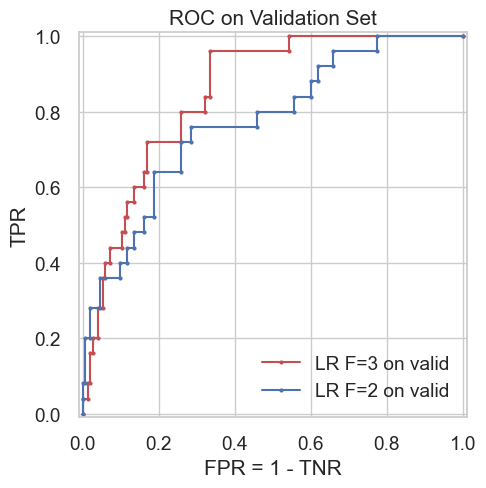
\includegraphics[width=0.75\textwidth]{fig1.png}  
    \caption{ROC curve with $F=3, F=2$}
    \label{fig:1}
\end{figure}

\subsection{Short answer}

At very high thresholds (high probability needed for cancer), we see the model
with 2 features report a higher ROC curve, and therefore higher performance.
For lower thresholds, we see the model with 3 features overtake the model with
2 features in performance. 

\begin{table}[h]
    \centering
    \resizebox{1\textwidth}{!}{%
    \begin{tabular}{|l|l|l|}
    \hline
                         & F=3 Logistic Regression with default threshold & F=3 Logistic Regression with best threshold \\ \hline
    Threshold used, $\tau$       &                      0.500                          &                     0.075                        \\ \hline
    Confusion Matrix     &                      
    \begin{tabular}{lrr}    
        Predicted & 0 & 1 \\
        True &  &  \\
        \midrule
        0 & 149 & 6 \\
        1 & 17 & 8 \\
        \end{tabular}                          &                  
        \begin{tabular}{lrr}
            Predicted & 0 & 1 \\
            True &  &  \\
            \midrule
            0 & 92 & 63 \\
            1 & 1 & 24 \\
            \end{tabular}                           \\ \hline
    TPR, TNR on test set &                  TPR = 0.320, TNR = 0.961	                              &                       TPR = 0.960, TNR = 0.594                      \\ \hline
    \end{tabular}%
    }
    \caption{Test-set performance for various Logistic Regression models}
\end{table}

\subsection{Short answer}
% (i) how many total patients in the test set would the classifier recommend
% not have a biopsy that would be done in current practice?
% (ii) how many of these skipped biopsies would result in good patient outcomes?
\begin{enumerate}[label=(\roman*)]
    \item If every patient in the test set would have had a biopsy in current
    practice, then all 180 patients would have had a biopsy. For any of the
    models, if the model predicts 0 (i.e. no cancer), then a biopsy is not
    considered necessary according to the model. 

    With the model selecting with the default threshold, we would see 149 + 17
    = \textbf{166 patients} who have been predicted to not have cancer. So,
    we do not perform a biopsy on \textbf{166 patients} in this situation. 

    With the model selecting with the best threshold, we would see 92 + 1 =
    \textbf{93 patients} who have been predicted to not have cancer. So, we do
    not perform a biopsy on \textbf{93 patients} in this situation.

    \item A good patient outcome is where we skipped a biopsy (predicted 0) and
    did not have cancer (true 0). This is a good outcome since the invasive procedure
    didn't have to happen, and we predicted that to be true. Suppose we didn't
    predict that to be true, then the biopsy would be for waste.

    For the model selecting with the default threshold, we have that
    \textbf{149 patients} have a good outcome. 

    For the model selecting with the best threshold, we have that \textbf{92
    patients} have a good outcome.
\end{enumerate} 

\subsection{Short answer}

    The best model for the doctors' goals is the logistic regression
    selecting with the best threshold (second model). 
   
    The first goal states that we don't want to send away a patient that
    actually had cancer. To avoid this, we want to reduce the amount of false
    negatives, and increase the amount of true positives. This corresponds
    directly to a higher $TPR  = \frac{TP}{TP\,+\, FN}$ since false negatives
    decreasing, and true positives increasing both make the TPR increase. Note
    that the TPR is better for the logistic regression selecting with the best
    threshold (second model) than the logistic regression selecting with the default
    threshold (first model). So, the second model achieves the first goal better
    than the first model. 

    Per the second goal, an unnecessary biopsy is when a patient is predicted
    to have cancer but does not end up being sick. This is a false positive in
    our classification system and a true 0 and predicted 1 in the confusion
    matrix. The model with the default threshold definitely has less
    patients with an unnecessary biopsy than the model with the best threshold.
    So, the default threshold model achieves the second goal for the doctors'
    better than the best threshold model.

    The default threshold model is still not better than the best threshold
    model. This is because in this situtation, less false negatives is far more
    important than less false positives. If we have more false negatives, we
    risk sending those who truly need treatment away. If we have more false
    positives, it's true that some procedures might be unnecessary, but we'd
    rather have less false negatives to ensure no one who truly has cancer does
    not get treated.

    For this reason, the second model, the logistic regression
    selecting with the best threshold, is the best model that achieves the
    doctors' goal.

\pagebreak
\subsection{Short answer}

\begin{figure}[htbp]
    \centering

    \begin{tabular}{lrr}
        \toprule
        Predicted & 0 & 1 \\
        True &  &  \\
        \midrule
        0 & 511.1 & 5.6 \\
        1 & 350.0 & 133.3 \\
        \bottomrule
        \end{tabular}
    
    \caption{Confusion matrix for 1000 samples of similar composition to test set using the Logistic Regression model with the best threshold}
    \label{fig:2}
\end{figure}

Note that the amount of biopsies that would be performed are any patients where
we predict 1, since our model suspects they have cancer. Also note that a life
threatening mistake is whenever we predict 0 for a patient, but truly have 1
for that patient.

So, in the \hyperref[fig:2]{confusion matrix above}, we see that we would
perform 5.6 + 133.3 = \textbf{138.9 biopsies}, in total. We would make 350.0
total life threatening mistakes (predicted 0, true 1).

\end{document}